\section{Introduction}
The gig economy has revolutionized delivery services, but existing platforms often prioritize customer convenience over courier well-being. LiftDrop addresses this gap by proposing a fairer, more efficient mobile app for deliveries.

\vspace{3mm}

\textbf{Key Goals:}

\begin{itemize}
    \item Optimize order assignment using real-time data (proximity, traffic, fairness)
    \item Enhance courier safety with neighborhood ratings and alerts
    \item Streamline operations via a scalable Android app backed by two APIs:
    \begin{itemize}
        \item \textbf{Courier API} (order management, real-time updates via SSE)
        \item \textbf{Client Simulation API} (mock orders for testing)
    \end{itemize}
\end{itemize}

\vspace{5mm}

The diagram below provides a high-level overview of LiftDrop's architecture:

\vspace{3mm}

\begin{figure}[h]
    \centering
    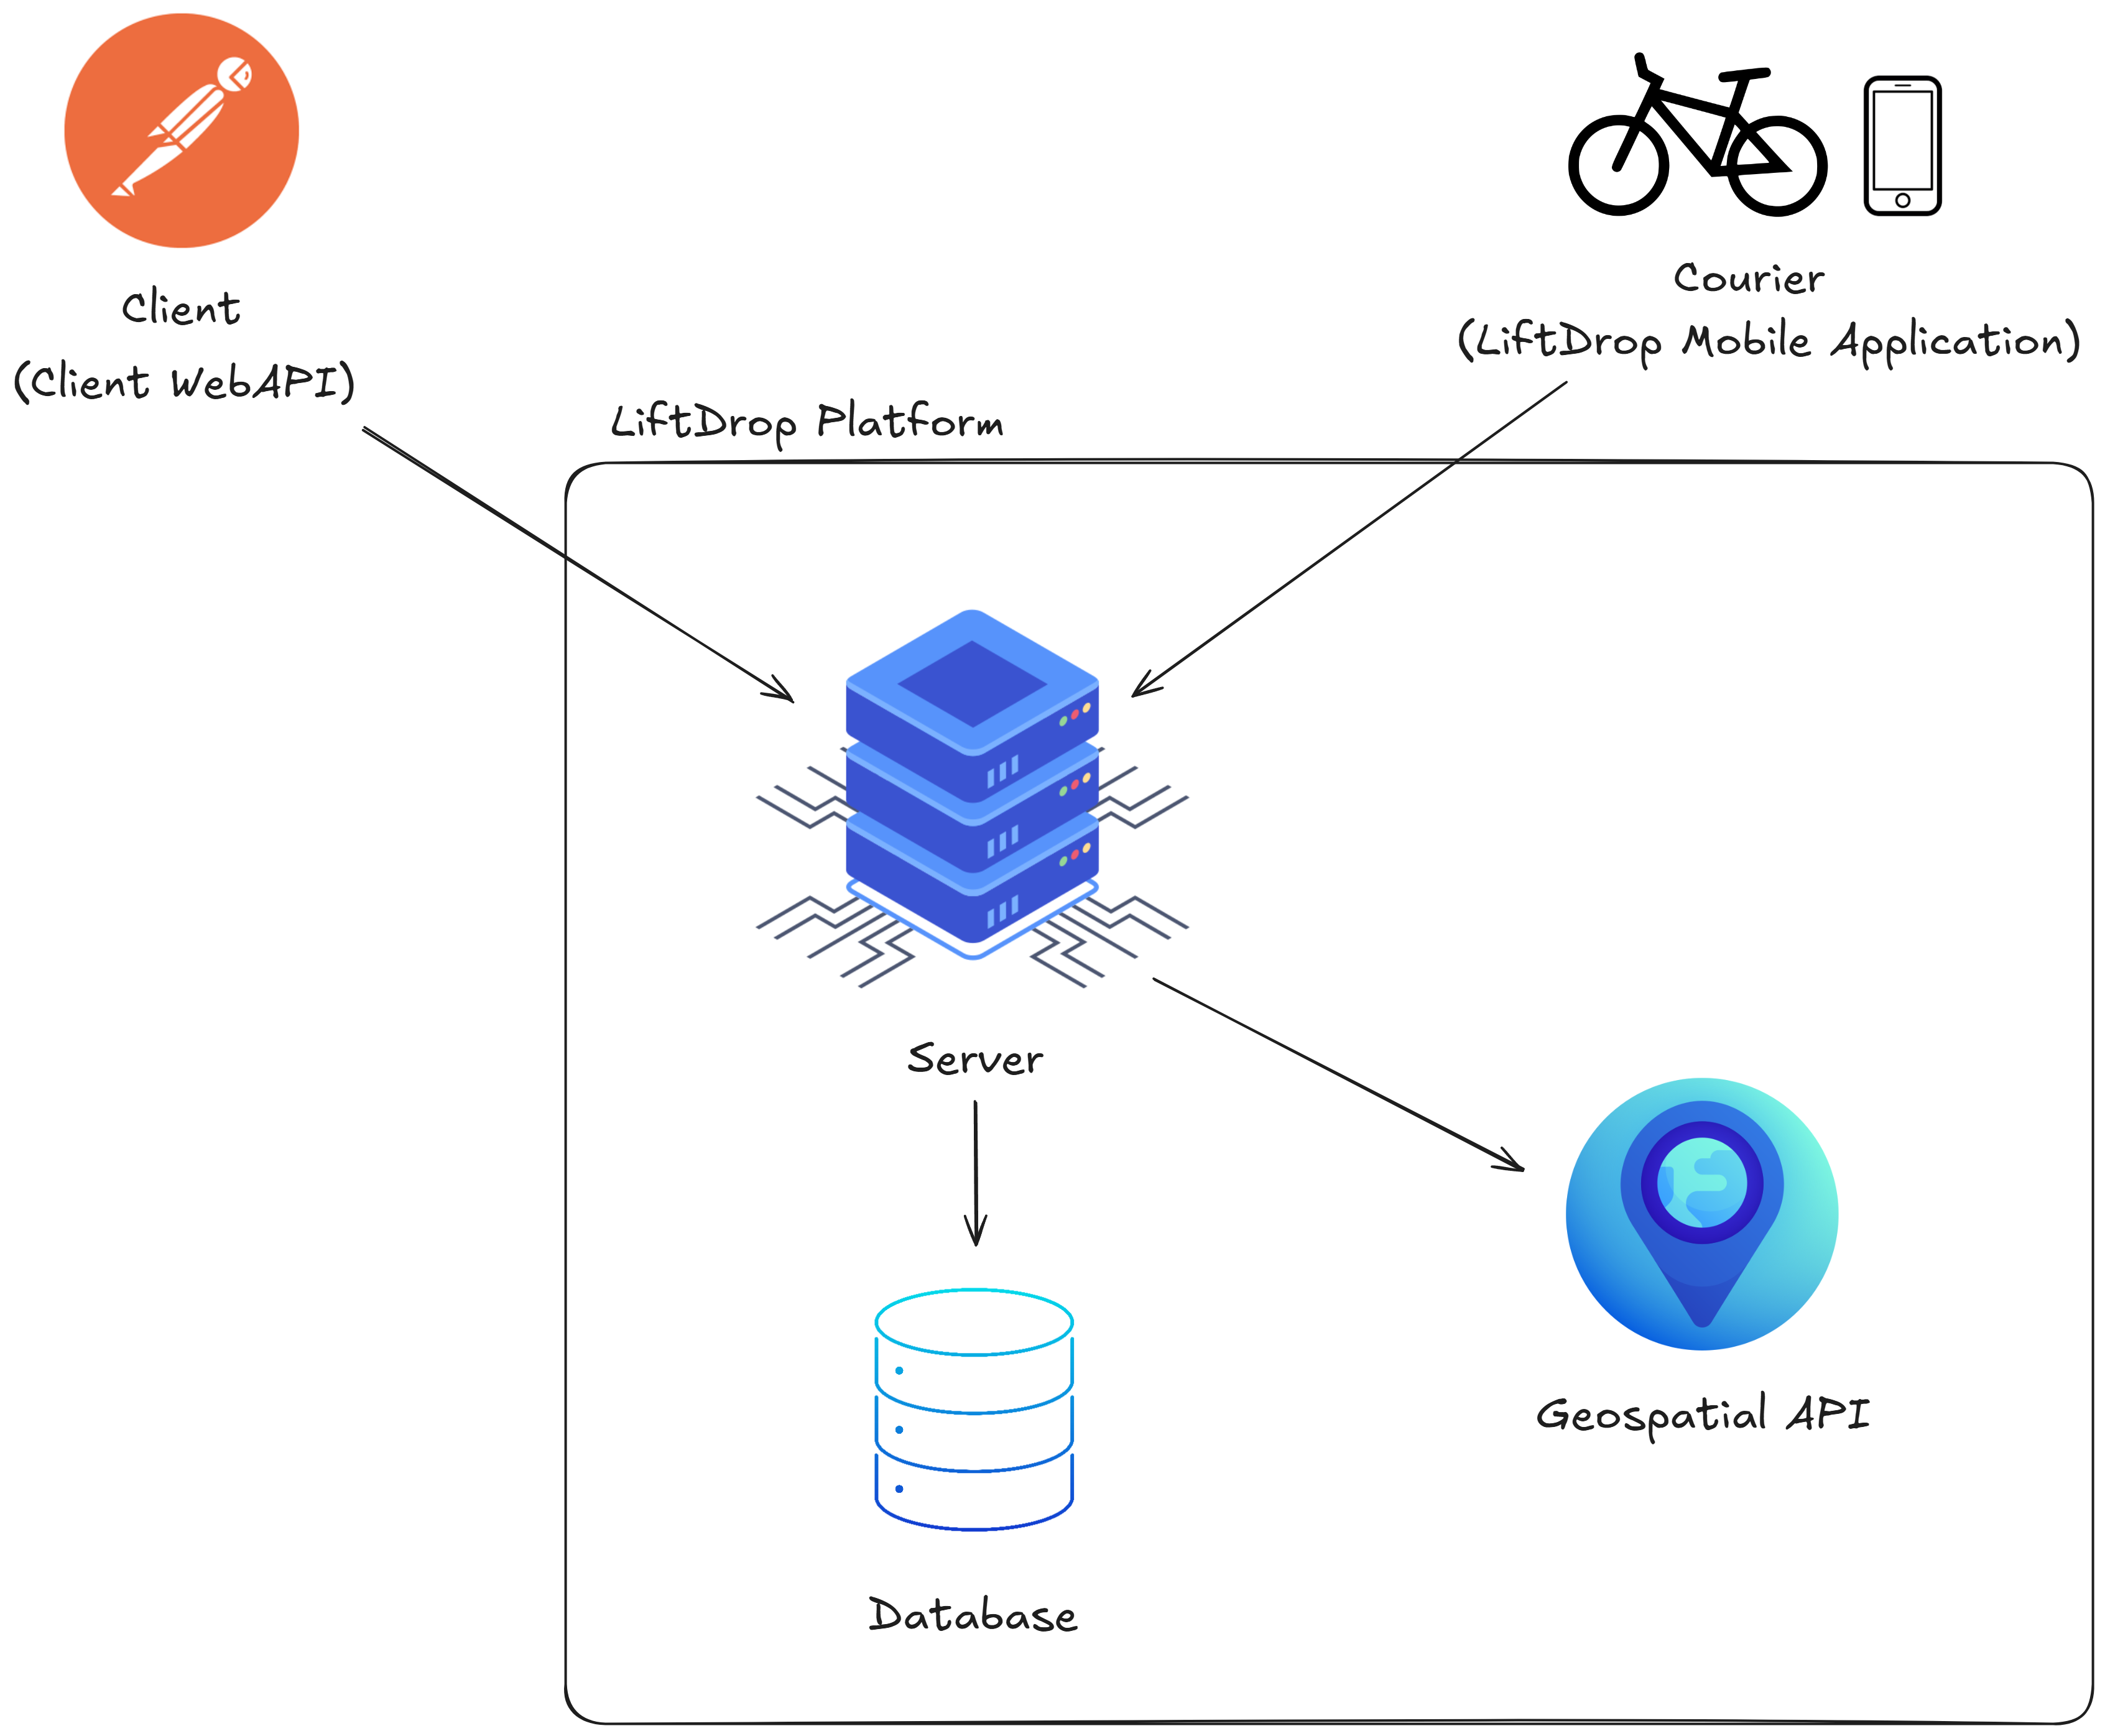
\includegraphics[width=0.8\textwidth]{images/LiftDrop_High_level_view.png}
    \caption{High-level overview of the platform, showing interaction between clients, server, database and external APIs (Google Maps).}
    \label{fig:high_level}
\end{figure}
